%% \chapter[htoc-titlei][hhead-titlei]{htitlei}
%% -----------------------------------------------------------------------------
\chapter[Theoretical overview][Theory]{Theoretical overview}
\label{ch:theory}

{\color{red} I'll need to go back and re-read through some books/papers before
  writing this chapter!}

{\color{red} Evelyn: 
keep this brief by referencing as much as possible.
Certainly contrast assumption of RPC vs assumption of RPV for experimental
searches.
Both are possibilities.
Stop as LSP does give unique (crazy?) signature not well
tested by previous searches (include LQ exclusion plot).
Could have different
decay rates to e, mu, tau.
}

In this chapter, a brief overview of the theoretical background for this thesis
is presented.
The topics discussed include the Standard Model (SM) of particle physics,
Supersymmetry, and the particular $B-L$ extension to the SM, which is the
focus of the search presented in this dissertation.
Additionally, the phenomenology of this $B-L$ extension is described.
In particular, the scenario where the scalar top is the LSP.
{\color{red}TODO add references to the following sections.}

%% ------------------------------------------------------------------------------
\FloatBarrier
\section{Standard Model}

The Standard Model (SM) of particle physics is described in
brief.
The SM is a quantum field theory which encapsulates the current understanding
of the elementary particles, and their interactions, and has been developed,
and rigorously tested over the last fifty years.
The interactions described by the Quantum Chromdynamics (QCD) and
electroweak sectors, are included in the SM Lagrangian, which is a non-abelian
gauge theory, with the symmetry group
$\mathrm{SU}(3)_\mathrm{c} \times \mathrm{SU}(2)_\mathrm{L} \times U(1)_\mathrm{Y}$.
% The SM Lagrangian describes matter and force carrier particles as quantum fields.
A more complete description of the SM can be found in
References~\cite{Agashe:2014kda,opac-b1131978,halzen1984quarks}.

The symmetry groups in the SM Lagrangian prescribe the particle content of the
force carriers.
Each of the force carrier fields have spin 1 (bosons), and are predicted to be
massless.
The QCD sector, with symmetry group $\mathrm{SU}(3)_\mathrm{c}$, contains eight
gluon fields, which mediate the interactions between particles with one of
three color charges {\color{red} TODO find references for QCD}.
The electroweak sector has the symmetry group,
$\mathrm{SU}(2)_\mathrm{L} \times U(1)_\mathrm{Y}$, and the interactions are
mediated by three $W^i$ boson fields, and a $B$ boson field.
The physical eigenstates of these fields are a mixture, leading to the
$W^{\pm}$ and $Z$ bosons, which mediate weak nuclear interactions, and the
photon ($\gamma$), which propagates electric fields
{\color{red} TODO find references for QCD}.

The matter particles are described in the SM Lagrangian as quantum fields, with
spin equal to \nicefrac{1}{2} (fermions).
The full list of fermions, and the corresponding quantum numbers shown
in Table~\ref{tab:sm_matter_content}.
The matter content is broken up into three generations of particles, each with
similar structure, differing by their mass.
Each generation includes quarks, which have both electric and color, change,
and therefore, interact with both the strong and electroweak forces.
Leptons, including charged leptons and neutrinos, are also included in each
generation, and have no color charge.
Charged leptons, such as electrons have electric charge, while neutrinos do not.

The weak force, mediated by the $W^{\pm}$ and $Z$ bosons, only interacts with
matter fields with left-handed chirality, with non-zero isospin.
In each generation, these left-handed fields make a quark doublet, comprising
an up and down type quark, and a lepton doublet, containing a neutrino and a
charged lepton.
These doublets behave the same way under weak interactions, with the up-type
quarks and neutrinos having the third component of weak isospin ($T_3$) equal 
to $+\nicefrac{1}{2}$, and the down-type quarks and charged leptons having
$T_3 = -\nicefrac{1}{2}$.
The quarks and charged leptons each have a corresponding right-handed particle.
These right-handed fermions are not part of an isospin doublet, and do not
interact via the weak force.
It should also be noted that, in the SM, neutrinos do not have a right-handed
counterpart, as they would not interact via any known forces.

\begin{table}
  \caption{Summary of the matter particles described by the SM, along with the
    associated quantum numbers.
    The quantum numbers include the spin, electric charge $Q$, the third
    component of weak isospin $T_3$, hypercharge $Y$, and the allowable color
    charges.
  }
  \label{tab:sm_matter_content}
  \begin{center}
    \begin{tabular}{ccccccccc}
      \toprule
      \multirow{2}{*}{Fermions} &
      \multicolumn{3}{c}{Generation} &
      \multirow{2}{*}{Spin} &
      \multirow{2}{*}{$Q$} &
      \multirow{2}{*}{$T_3$} &
      \multirow{2}{*}{$Y$} &
      \multirow{2}{*}{Color}
      \\[1ex]
      & 1 & 2 & 3
      \\
      \midrule
      \addlinespace[1ex]
      %%
      \multirow{5}{*}{Quarks} &
      \multirow{2}{*}{$\left(
          \begin{tabular}{c} u \\ d \end{tabular} \right)_{L}$ } &
      \multirow{2}{*}{$\left(
          \begin{tabular}{c} c \\ s \end{tabular} \right)_{L}$ } &
      \multirow{2}{*}{$\left(
          \begin{tabular}{c} t \\ b \end{tabular} \right)_{L}$ } &
      \multirow{2}{*}{$\frac{1}{2}$} &
      $+\frac{2}{3}$ &
      $+\frac{1}{2}$ &
      \multirow{2}{*}{$\frac{1}{6}$} &
      \multirow{2}{*}{r, g, b}
      \\[1ex]
      %%
      & & & & &
      $-\frac{1}{3}$ &
      $-\frac{1}{2}$ &
      &
      \\
      %%
      \cmidrule{2-9}
      %%
      &
      $u_R$ &
      $c_R$ &
      $t_R$ &
      $\frac{1}{2}$ &
      $+\frac{1}{2}$ &
      0 &
      $+\frac{2}{3}$ &
      r, g, b
      \\[1ex]
      %%
      &
      $d_R$ &
      $s_R$ &
      $b_R$ &
      $\frac{1}{2}$ &
      $-\frac{1}{2}$ &
      0 &
      $-\frac{1}{3}$ &
      r, g, b
      \\
      %%
      \midrule
      %%
      \multirow{3}{*}{Leptons} &
      \multirow{2}{*}{$\left(
          \begin{tabular}{c} $\nu_{e}$ \\ e \end{tabular}
        \right)_{L}$ } &
      \multirow{2}{*}{$\left(
          \begin{tabular}{c} $\nu_{\mu}$ \\ $\mu$ \end{tabular}
        \right)_{L}$ } &
      \multirow{2}{*}{$\left(
          \begin{tabular}{c} $\nu_{\tau}$ \\ $\tau$ \end{tabular}
        \right)_{L}$ } &
      \multirow{2}{*}{$\frac{1}{2}$} &
      0 &
      $+\frac{1}{2}$ &
      \multirow{2}{*}{-$\frac{1}{2}$} &
      \multirow{2}{*}{-}
      \\[1ex]
      %%
      & & & & &
      $-1$ &
      $-\frac{1}{2}$ &
      &
      \\
      \cmidrule{2-9}
      %%
      &
      $e_{R}$ &
      $\mu_{R}$ &
      $\tau_{R}$ &
      $\frac{1}{2}$ &
      $-1$ &
      0 &
      $-1$ &
      -
      \\
      \bottomrule
    \end{tabular}
  \end{center}
  
\end{table}

%% - - - - - - - - - - - - - - - - - - - - - - - - - - - - - - - - - - - - - - -
\FloatBarrier
\subsection{Higgs mechanism}

While the photon is a massless particle, the $W^{\pm}$ and $Z$ bosons are
observed to be short ranged, implying they are massive.
The addition of these mass terms breaks gauge invariant in the SM Lagrangian,
and is, therefore, forbidden.
Similarly, the fermions have masses, which are forbidden by the SM.
This would allow a mixing between the left- and right-handed fermions,
which would break gauge invariance.

A method to add mass terms to the SM Lagrangian without breaking the necessary
gauge invariance was developed during the 1960's by several groups of theorists,
including Robert Brout and Francois Englert~\cite{PhysRevLett.13.321},
Peter Higgs~\cite{Higgs1964132,PhysRevLett.13.508},
and Gerald Guralnik, Carl R. Hagen, and Tom Kibble~\cite{PhysRevLett.13.585}
working in parallel, and is commonly called the Brout-Englert-Higgs (BEH)
mechanism.
The BEH mechanism adds an additional complex scaler field, known as the Higgs
field, to the Lagrangian, for which the ground state of the field is not at its
zero-point.
The Higgs field ``spontaneously'' breaks the gauge symmetry while preserving
the gauge invariance of the Lagrangian.

%% -----------------------------------------------------------------------------
\FloatBarrier
\section{Supersymmetry}

Lightest supersymmetric particle (LSP) 

%% - - - - - - - - - - - - - - - - - - - - - - - - - - - - - - - - - - - - - - -
\subsection{R-Parity}

The extension of the Standard Model of particle physics with
supersymmetry (SUSY)~\cite{Miyazawa:1966,Ramond:1971gb,Golfand:1971iw,
Neveu:1971rx,Neveu:1971iv,Gervais:1971ji,Volkov:1973ix,Wess:1973kz,Wess:1974tw}
immediately leads to processes that violate both baryon number ($B$) and
lepton number ($L$), leading to rapid proton decay and
lepton-number-violating processes, such as unseen decays of
$\mu \to e\gamma$, in conflict with experimental bounds.
A conventional assumption to prevent these processes is to impose
conservation of $R$-parity~\cite{Fayet:1976et,Fayet:1977yc,Farrar:1978xj,
Fayet:1979sa,Dimopoulos:1981zb},
defined as $R=(-1)^{3(B-L)+2s}$ where $s$ is the spin of the particle.
This has a value of $+1$ for Standard Model particles and $-1$ for
SUSY particles.
In this case SUSY particles are produced in pairs, and the LSP is stable.
Further, this stable LSP cannot carry electric charge or color charge without
coming into conflict with astrophysical data.
At the LHC, the conventional experimental signature for SUSY particles
includes significant missing transverse momentum due to the non-interaction of
the LSP with the detector.

%% -----------------------------------------------------------------------------
\FloatBarrier
\section{B-L extension}
\label{sec:theory_bl_extension}


%% - - - - - - - - - - - - - - - - - - - - - - - - - - - - - - - - - - - - - - -
\FloatBarrier
\subsection{Motivation}

{\color{red} Why this model? :-) Talk about things like:
\begin{itemize}
\item RPC is overkill to prevent proton decay
\item Links neutrino sector to susy properties
\end{itemize}
}

An alternative approach is to add a local symmetry $U(1)_{B-L}$ to the
$SU(3)_C \times SU(2)_L \times U(1)_Y$ Standard Model with right-handed
neutrinos.
The minimal supersymmetric extension then only needs a vacuum expectation value
for a right-handed sneutrino in order to spontaneously break the
$B-L$ symmetry~\cite{FileviezPerez:2008sx, Barger:2008wn, FileviezPerez:2009gr,
Everett:2009vy, Evans:1986ada, Lukas:1998yy, Braun:2005ux, Braun:2005nv,
Braun:2006ae, Ambroso:2009jd, Ambroso:2010pe, Ovrut:2012wg}.
This minimal $B-L$ model violates lepton number but not baryon number, and is
consistent with proton stability and the bounds on lepton number violation.
The LSP can now decay via $R$-parity-violating (RPV) processes, and may now
carry color and electric charge.

%% - - - - - - - - - - - - - - - - - - - - - - - - - - - - - - - - - - - - - - -
\FloatBarrier
\subsection{Phenomenology}

This leads to unique signatures~\cite{FileviezPerez:2012mj, Perez:2013kla,
Ovrut:2012wg, Ovrut:2014rba, Ovrut:2015uea} that are disallowed in conventional
models with $R$-parity conservation.
The case where the LSP is a scalar top (stop) is most interesting
since, in general, the large mass of the top quark acts to make the
lightest stop significantly lighter than the other squarks due to
renormalization group effects~\cite{Barbieri:1987fn,deCarlos:1993yy}.
The stop decays via an RPV interaction to a charged lepton (of any
flavor) and a $b$-quark.
The decay branching fractions to $e b$, $\mu b$, and $\tau b$ may be different,
in a manner related to the neutrino mass
hierarchy seen in Figure~\ref{fig:pheno_bounds}.
Each point in this plot represents a simulation with a particular choice of
model parameters, all varied within a natural range of values, shown in
Table~\ref{tab:pheno_ranges}, and the four colors represent different choices
for the neutrino mass hierarchy and 
$\sin^2\theta_{23}$~\cite{Marshall:2014cwa,Marshall:2014kea}.
There is a clear relation between the neutrino mass hierarchy and the allowed
stop branching ratios, therefore if a stop consistent with this model is
discovered, its properties could potentially give information about the
structure of the neutrino sector.

\begin{figure}[p]
  \centering{
    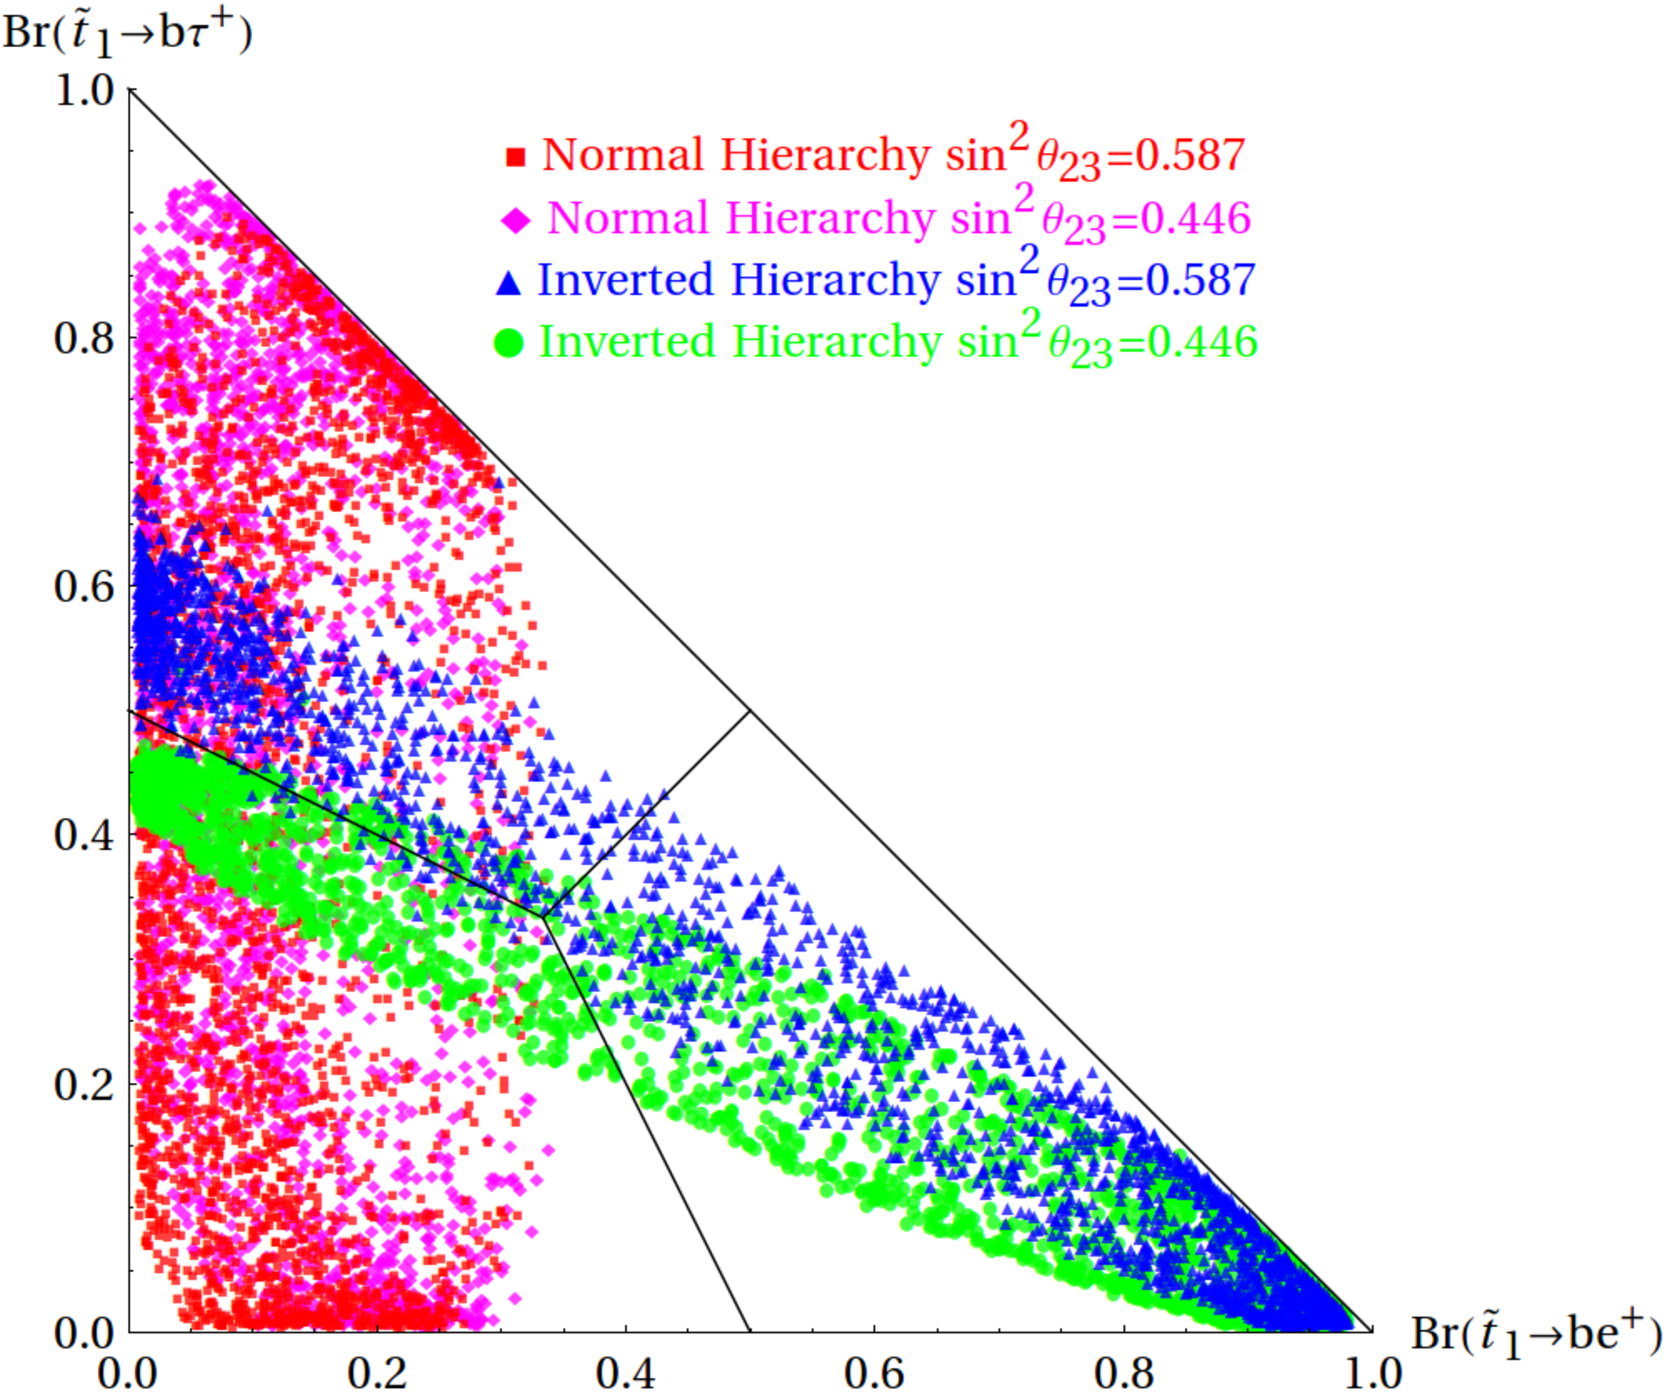
\includegraphics[width=\textwidth]{figs/theory/WithGaussian.pdf}
    \caption{This plot shows the allowed branching ratios for the stop LSP
      for various choices of the neutrino mass hierarchy and
      $\sin^2\theta_{23}$,
      obtained by varying various model parameters within a range of natural
      values shown in Table~\ref{tab:pheno_ranges}~\cite{Marshall:2014cwa}.
    }
    \label{fig:pheno_bounds}
  }
\end{figure}

\begin{table}[ht]
  \caption{Ranges for the parameter scan used to generate the simulated models
    in \cref{fig:stop_vs_mixing_angle,fig:pheno_bounds}.
    The neutrino sector constrains all buy one one of the R-parity violating
    parameters, which is chosen to be $\epsilon_i$ where the generational
    index, $i$, is also scanned to avoid any biases.
    ``NH'' and ``IH'' represent the normal and inverted neutrino mass hierarchy
    respectively~\cite{Marshall:2014cwa}.
  }
  \label{tab:pheno_ranges}
  \centering{
    \begin{tabular}{cc}
      \toprule
      Parameter & Range \\
      \midrule
      $M_3~[\TeV]$               & $1.5 - 10$    \\[1ex]
      $M_{Z_\mathrm{R}}~[\TeV]$  & $2.5 - 10$    \\[1ex]
      $\tan\beta$                & $2 - 55$      \\[1ex]
      $\mu~[\GeV]$               & $150 - 1000$  \\[1ex]
      $m_{\stop_1}~[\GeV]$       & $400 - 1000$  \\[1ex]
      $\theta_t~[^\circ]$        & $0 - 90$      \\[1ex]
      $|\epsilon_i|~[\GeV]$      & $10^{-4} - 1$ \\[1ex]
      $\arg(\epsilon_i)$         & $0 - 360$     \\[1ex]
      $i$                        & $1 - 3$       \\[1ex]
      $\xi_0, \xi_3$             & $-1, 1$       \\[1ex]
      $\delta,\alpha~[^{\circ}]$ & $0 - 360$     \\[1ex]
      Neutrino Hierarchy         & NH, IH        \\
      \bottomrule
    \end{tabular}
  }
\end{table}

Within this model, a stop LSP can decay in one of two ways, depending on
the handedness of the stop.
A right-handed stop decays to a top quark and a right-handed neutrino with a
coupling strength proportional to vacuum expectation value (VEV) of the
left-handed neutrino mass.
This must be small because the left-handed sneutrino interacts with the
$W$ and $Z$ bosons, and a large VEV would result in these bosons gaining
additional mass.
{\color{red} (TODO check this statement is true - I think I'm missing
something).}
A purely left-handed stop decays to a $b$-quark and a lepton with the coupling
strength proportional to the VEV of the right-handed sneutrino, which may be
large, as the right-handed sneutrino does not couple to the electroweak bosons,
a large VEV does not break electroweak symmetry.
{\color{red} (TODO check this statement is true - I think I'm missing
something)}.
In the scenario where the stop LSP is an admixture of left- and right-handed
stops, the preferred decay mode depends on the stop mixing angle ($\theta_t$).
This dependence is plotted in Figure~\ref{fig:stop_br_vs_mixing_angle}, which
shows the ratio
$\nicefrac{\mathrm{Br}(\stop \to t\nu)}{\mathrm{Br}(\stop \to b\ell)}$
versus $\theta_t$.
Each point represents a simulation with a particular choice of model parameters,
again scanning over the natural values in Table~\ref{tab:pheno_ranges}.
The $\stop \to b\ell$ decay is the dominant decay mode for mixing angles less
than abut $80^{\circ}$, where the LSP stop is mostly right handed, and the
$\stop \to t\nu$ decay becomes significance.
The $\stop \to b\ell$ decay is still non-negligible for a mostly right-handed
stop in many of the simulated models,
however~\cite{Marshall:2014cwa,Marshall:2014kea}.

\begin{figure}[ht]
  \centering{
    \subbottom[Stop branching ratio]{
      % 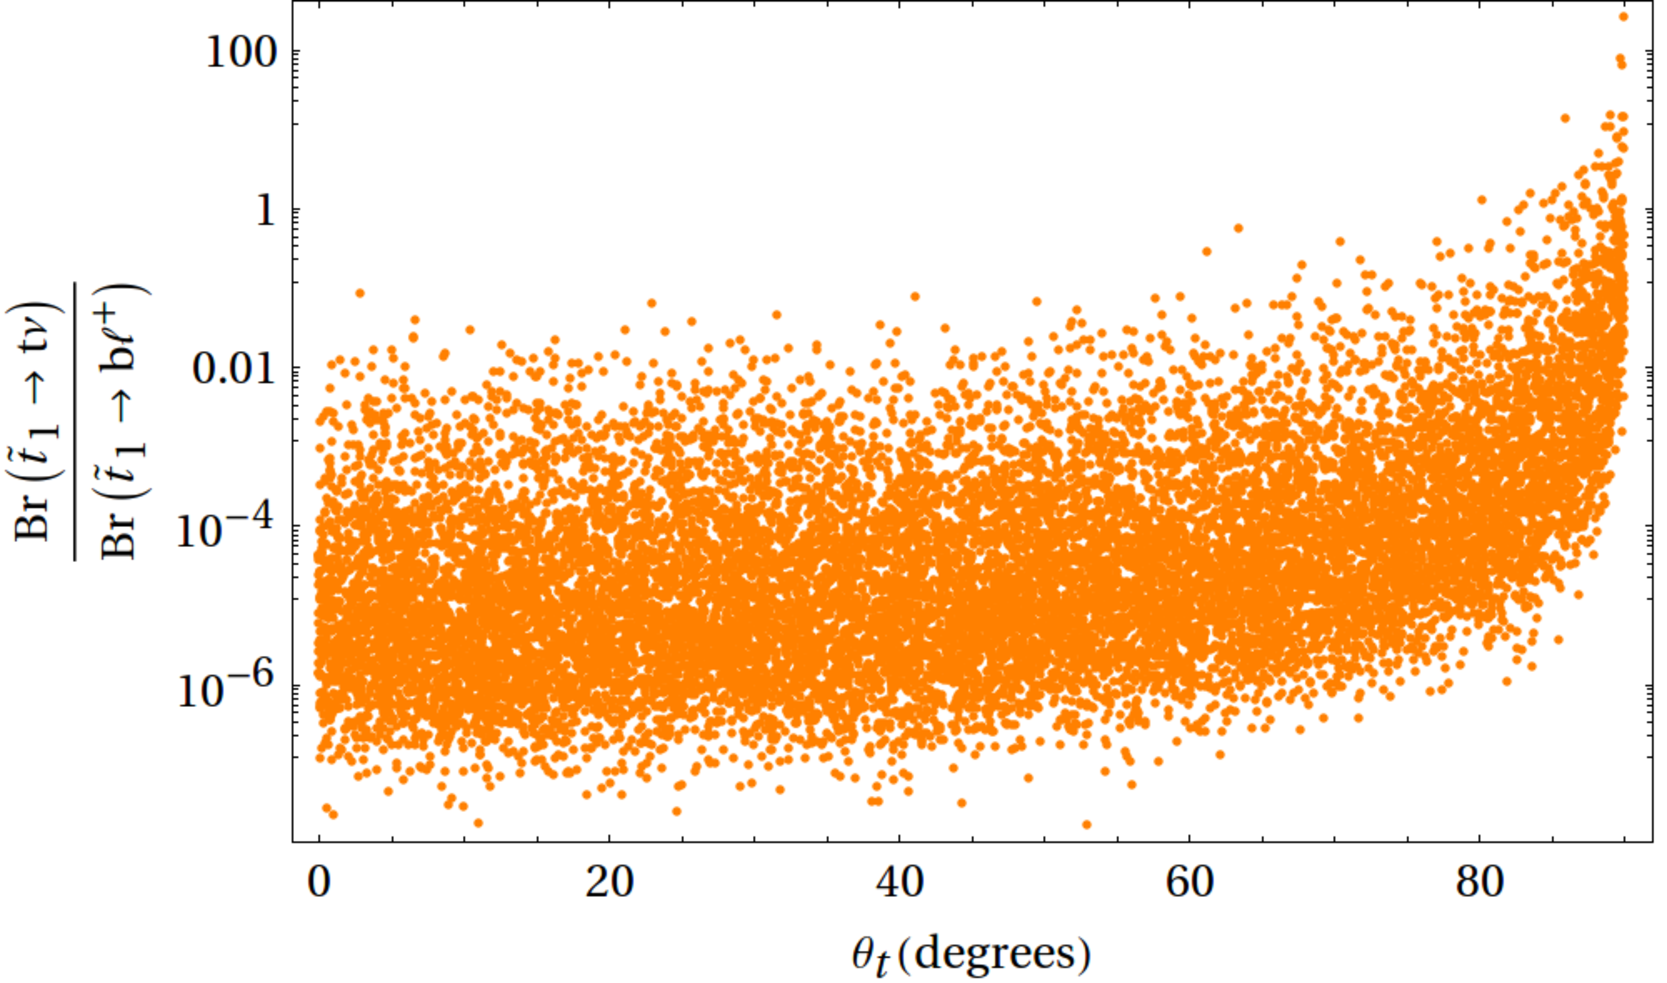
\includegraphics[width=0.70\textwidth]{figs/theory/StopBranchingRatiosVsMixingAngle.pdf}
      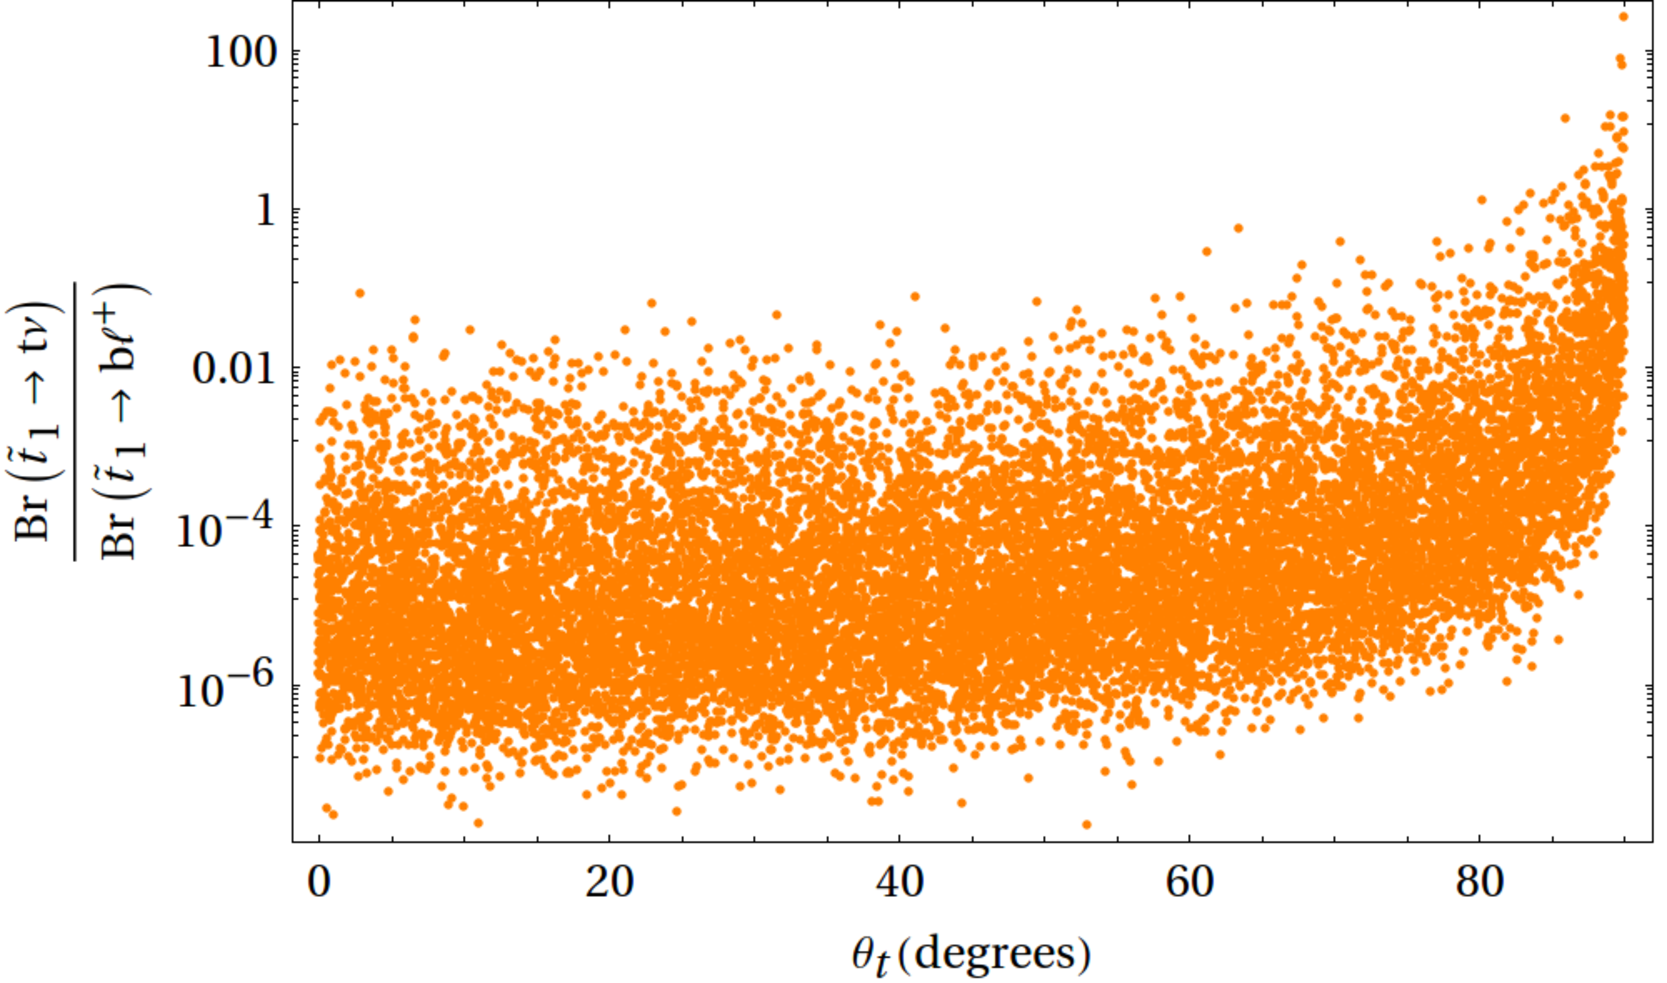
\includegraphics[width=\textwidth]{figs/theory/StopBranchingRatiosVsMixingAngle.pdf}
      \label{fig:stop_br_vs_mixing_angle}
    }
    \subbottom[Stop decay length]{
      % 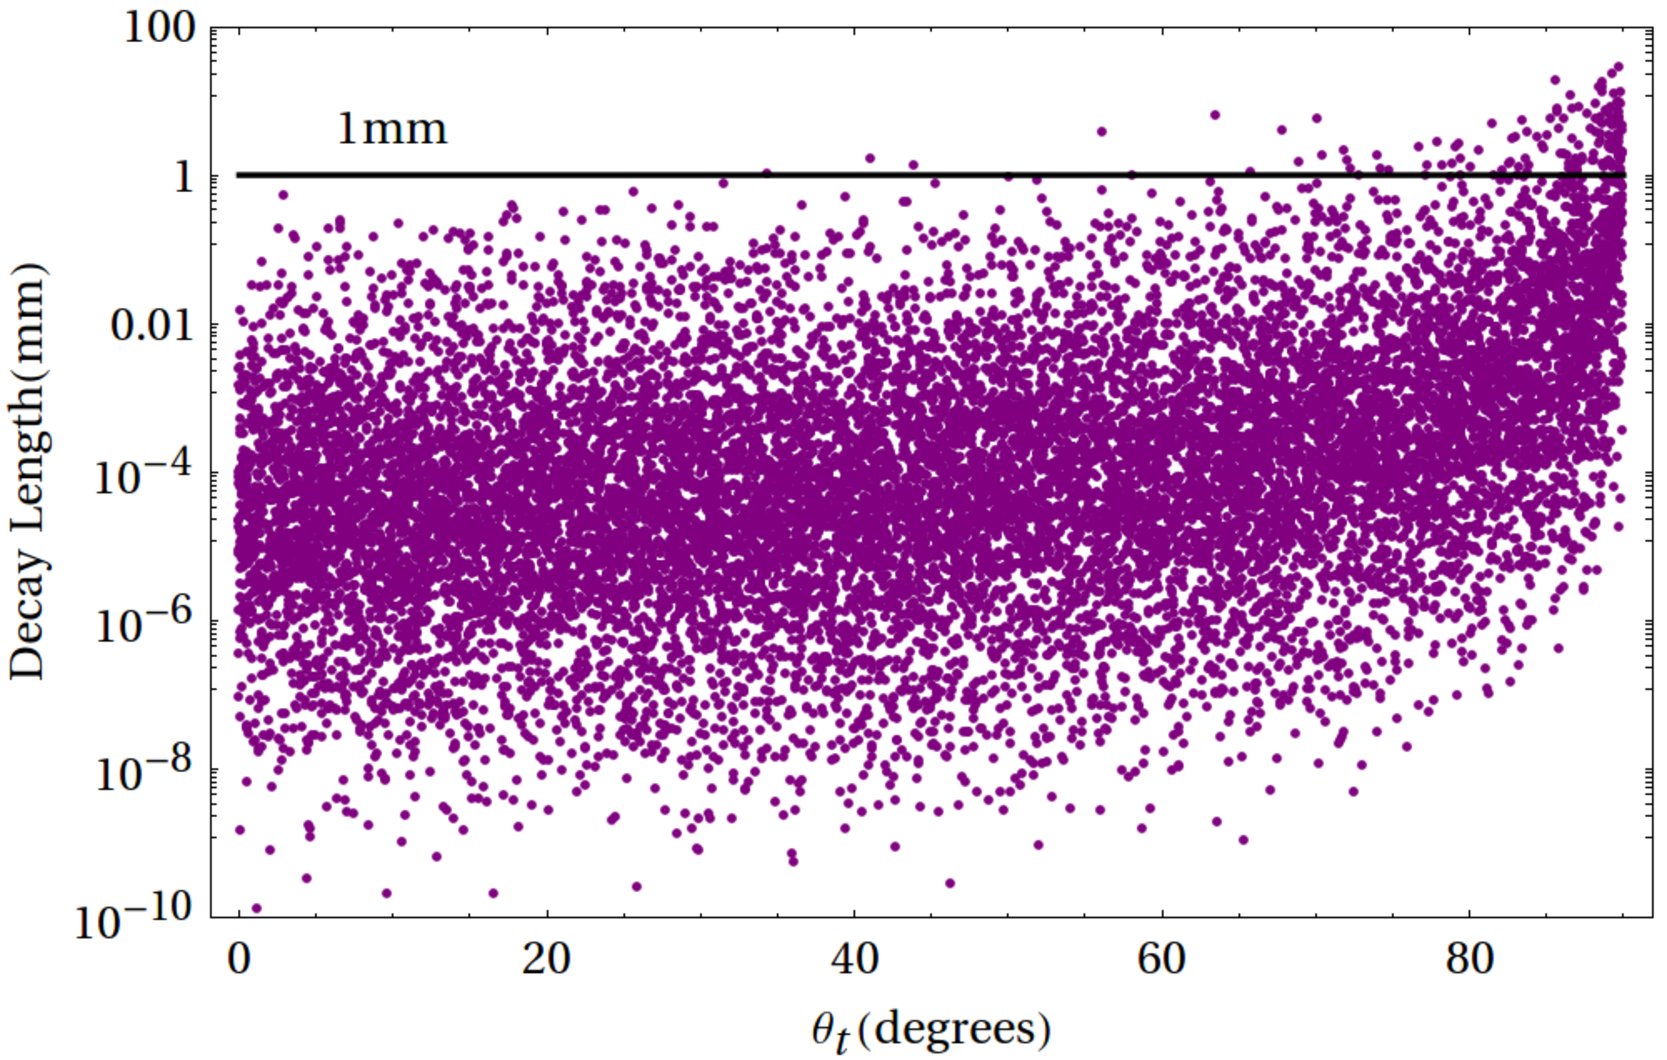
\includegraphics[width=0.70\textwidth]{figs/theory/DecayLength.pdf}
      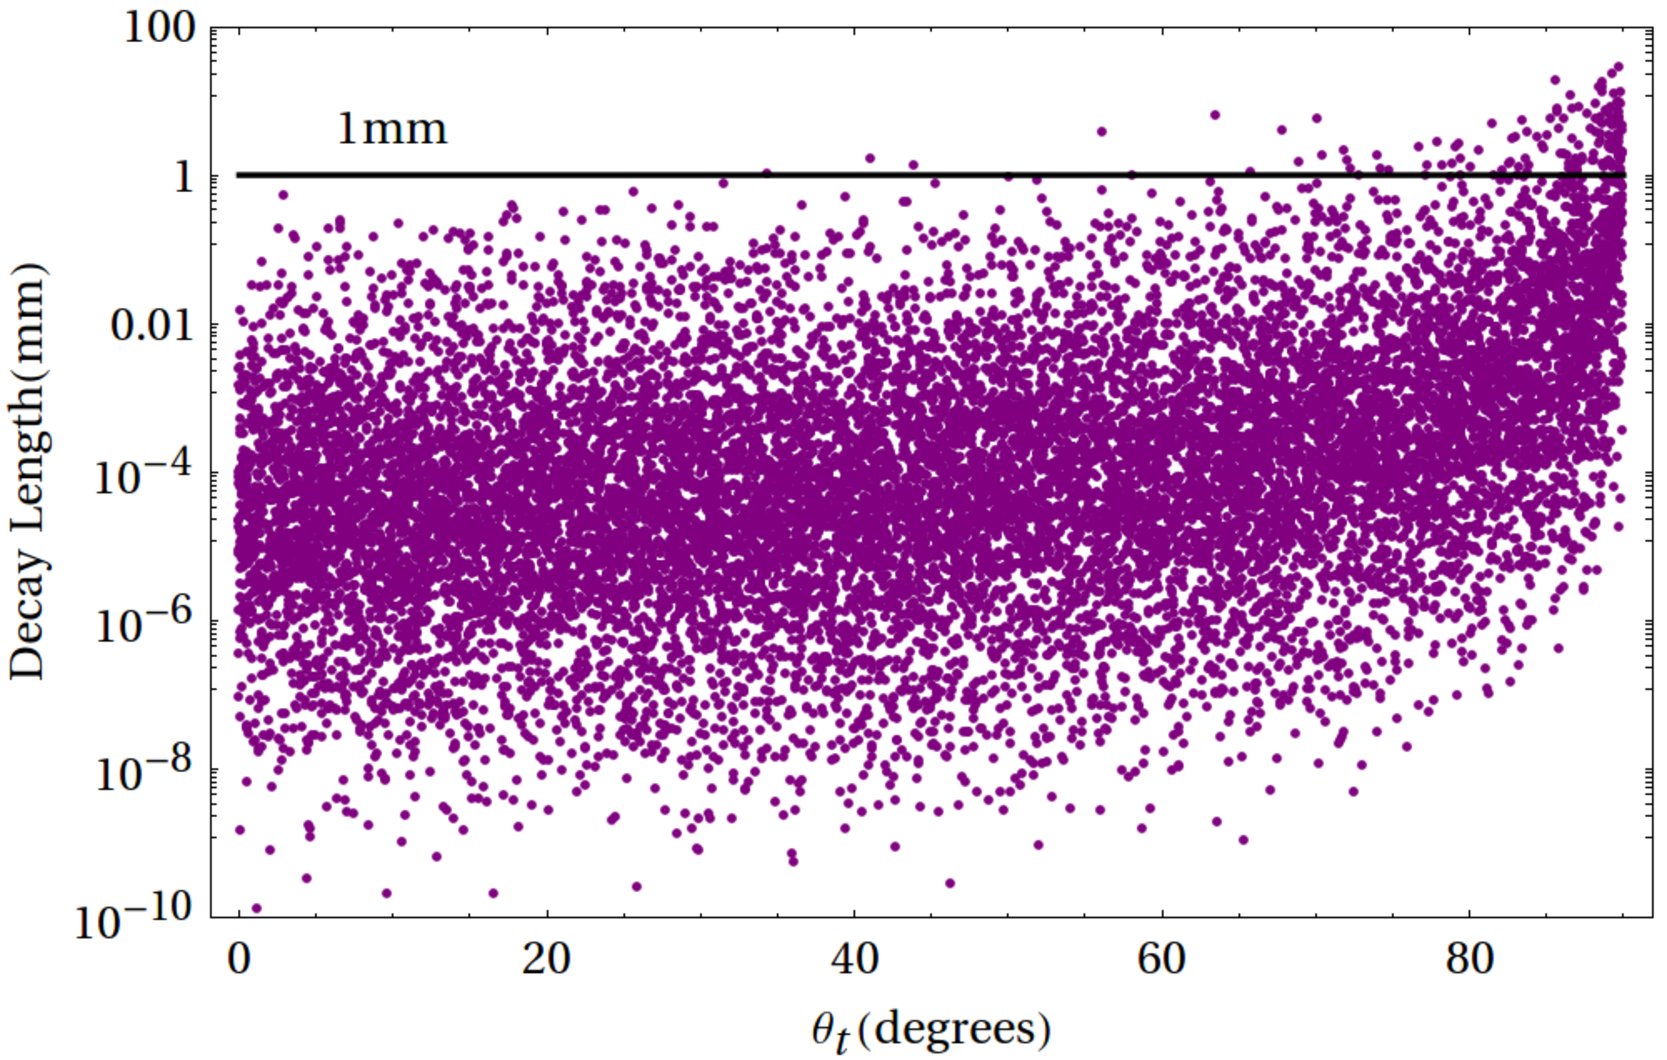
\includegraphics[width=\textwidth]{figs/theory/DecayLength.pdf}
      \label{fig:stop_decay_length_vs_mixing_angle}
    }
    \caption{These plots show the stop decay length and branching ratio versus
      the stop mixing angle, assuming the stop is the LSP.
      Each point in these plots represent a simulation with a particular
      choice of model parameters, which are varies within a range of natural
      values~\cite{Marshall:2014cwa}.
    }
    \label{fig:stop_vs_mixing_angle}
  }
\end{figure}

The analysis described in this thesis focuses on the $\stop \to b\ell$ decay
as it is preferred for most of parameter space.
Additionally, if the $\stop \to t\nu$ decay is significant, the decay of stop
pairs would lead to final states with $t\bar{t}$ associated with large missing
energy, which is the same final state as stop pair production with
$R$-Parity conserving decays, and the limits from traditional stop searches can
be reinterpreted for this model.

It is also reasonable to assume the stop decays in this model are prompt, and
decay with a negligible impact parameter, as shown in
Figure~\ref{fig:stop_decay_length_vs_mixing_angle}, where for most natural
models, the stop is expected to have a decay length of less than
$10^{-3}~\mathrm{mm}$;
in particular, this is true for models where the stop is not mostly
right-handed ($\theta_t \leq 80$)~\cite{Marshall:2014cwa,Marshall:2014kea}.
Therefore, long-lived particles are not considered in this analysis.

In this $B-L$ extension to the MSSM, stop pair production has the same
production cross section as in the traditional MSSM.
The expected production cross section are shown in Figure~\ref{fig:stop_xsec}.

\begin{figure}[ht]
  \centering{
    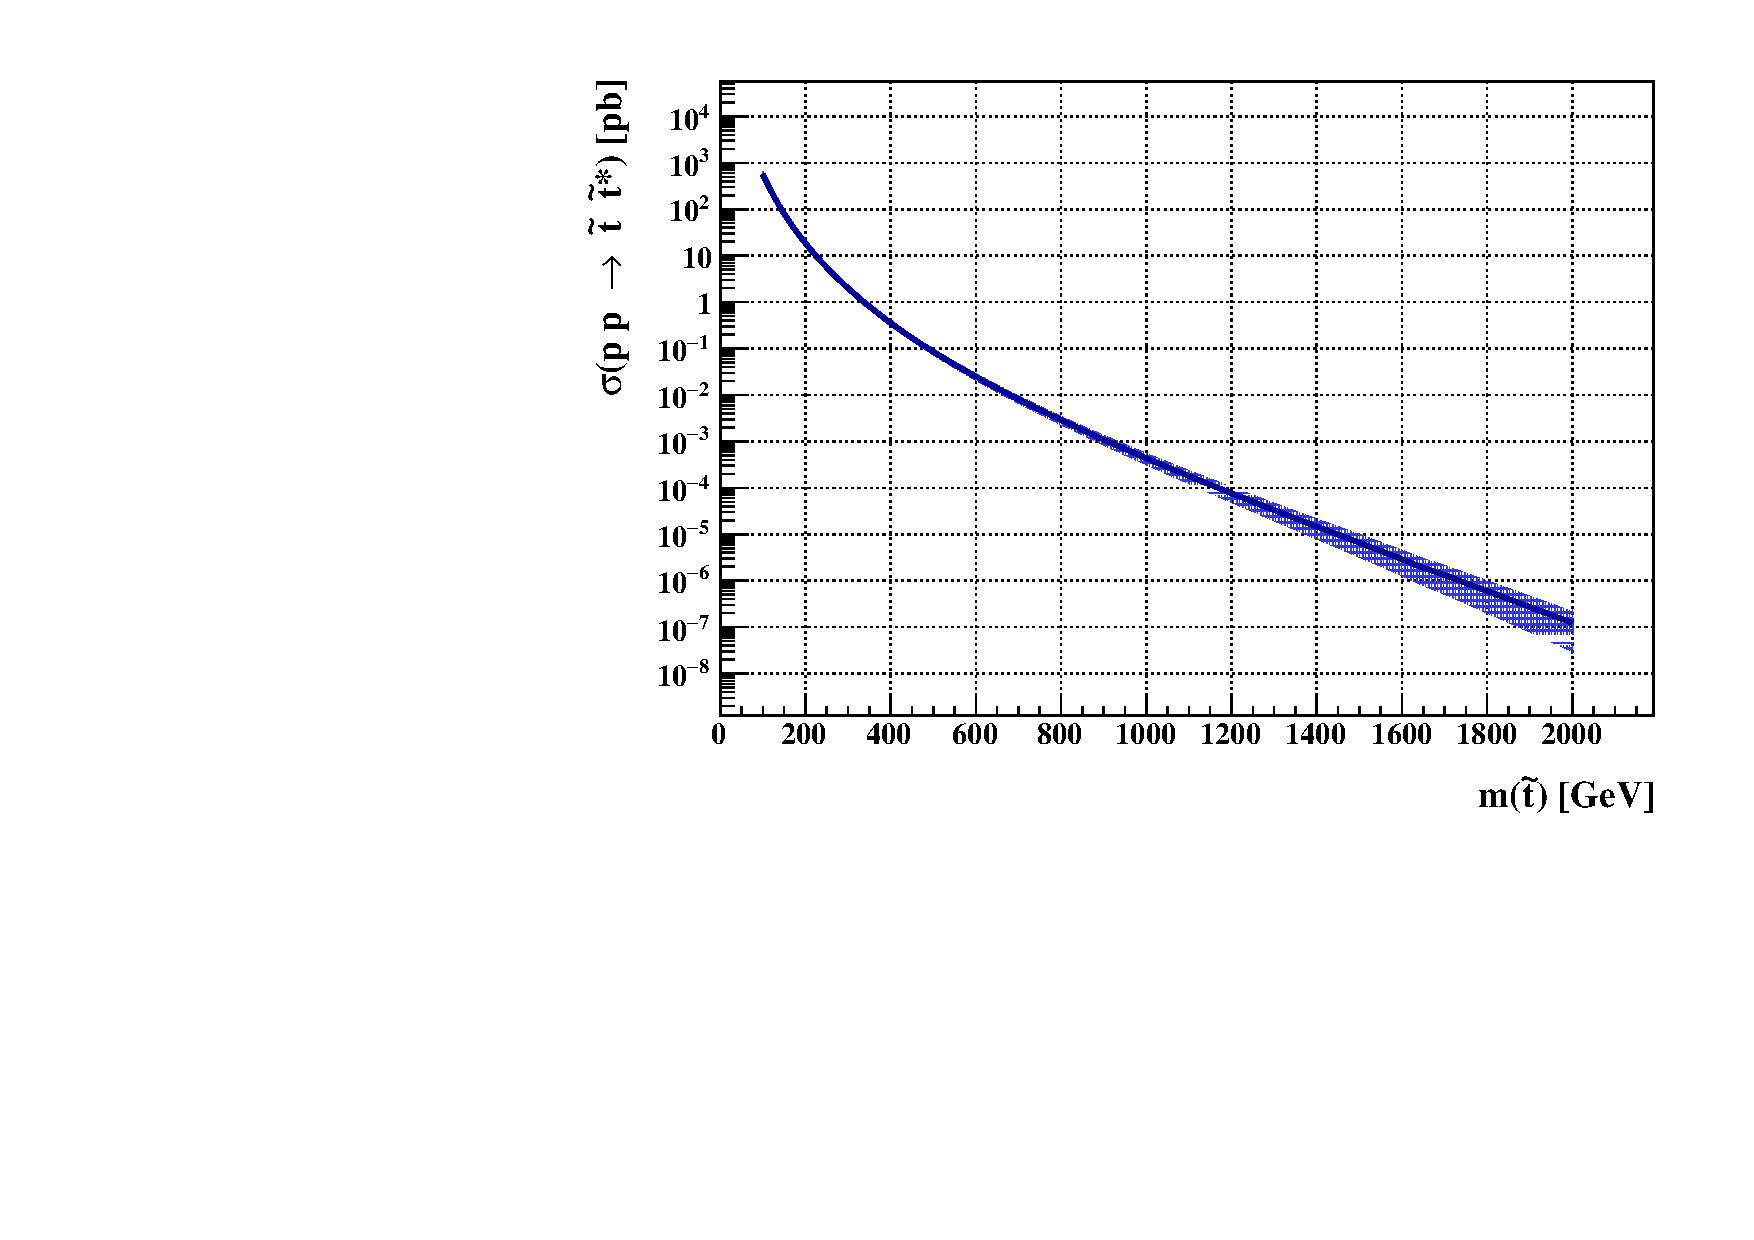
\includegraphics[width=\textwidth]{figs/theory/xsec.pdf}
  }
  \caption{Stop cross sections and their associated
    uncertainties~\cite{Beenakker:1997ut,Beenakker:2010nq,Beenakker:2011fu}.
  }
  \label{fig:stop_xsec}
\end{figure}

% %% -----------------------------------------------------------------------------
% \FloatBarrier
% \subsection{Expected kinematics}
% 
% {\color{red} TODO talk about expected event kinematics at truth level}
% 
% The expected event kinematics are studied using Monte Carlo (MC) simulation.
% Simulated stop pair production events are generated using \madgraph\ version
% 1.5.12~\cite{Alwall:2011uj} and \pythia\ version 6.427~\cite{Sjostrand:2006za},
% and the expected event kinematics are studied at the truth level, ignoring
% detector effects and potential inefficiencies.
% The simulated signal event generation procedure is described in more detail in
% Section~\ref{sec:mc_samples}.
% For illustration purposes, three choices of stop mass (100~\GeV, 500~\GeV,
% and 1000~\GeV), are compared in this section to give a picture of how the event
% kinematics are expected to evolve with increasing stop mass.
% 
% Figure~\ref{fig:truth_stop_pt} shows the expected 

%% -----------------------------------------------------------------------------
\FloatBarrier
\subsection{Previous results}

The results from existing leptoquark searches performed at ATLAS were
re-interpreted in the context of this $B-L$ SUSY model with a stop LSP, and the
limits obtained on the minimum allowable stop mass across the plane of
physical stop branching ratios are shown in
Figure~\ref{fig:pheno_limit}~\cite{Marshall:2014cwa,Marshall:2014kea}.
The leptoquark searches, used to obtain these mass limits, searched for
models where the decay products are in the same generation.
As a result, $b$-tagging is only required in events associated with a $\tau$
lepton, and events with a light lepton simply require a jet, regardless of the
flavor.
Additionally, previous leptoquark searches only consider decays to a single
lepton flavor, resulting in final states with either two leptons of the same
flavor and two jets, or a single charged lepton and at least one jet.
The previous analyses did not consider final states with two charged leptons
with different flavors ($e\mu$) and at least two 
jets~\cite{ATLAS:2013oea, ATLAS:2012aq, Aad:2011ch, CMS:2014qpa,
  Chatrchyan:2012sv, Chatrchyan:2012vza, Chatrchyan:2012st}.
A dedicated search requiring $b$-tagged jets associated with light leptons
(electrons and muons), and considering different flavored leptons in the final
state can provide additional sensitivity to this model, as well as other models
which result in final states with $b$-quarks and light leptons in the final
state.

\begin{figure}[p]
  \centering{
    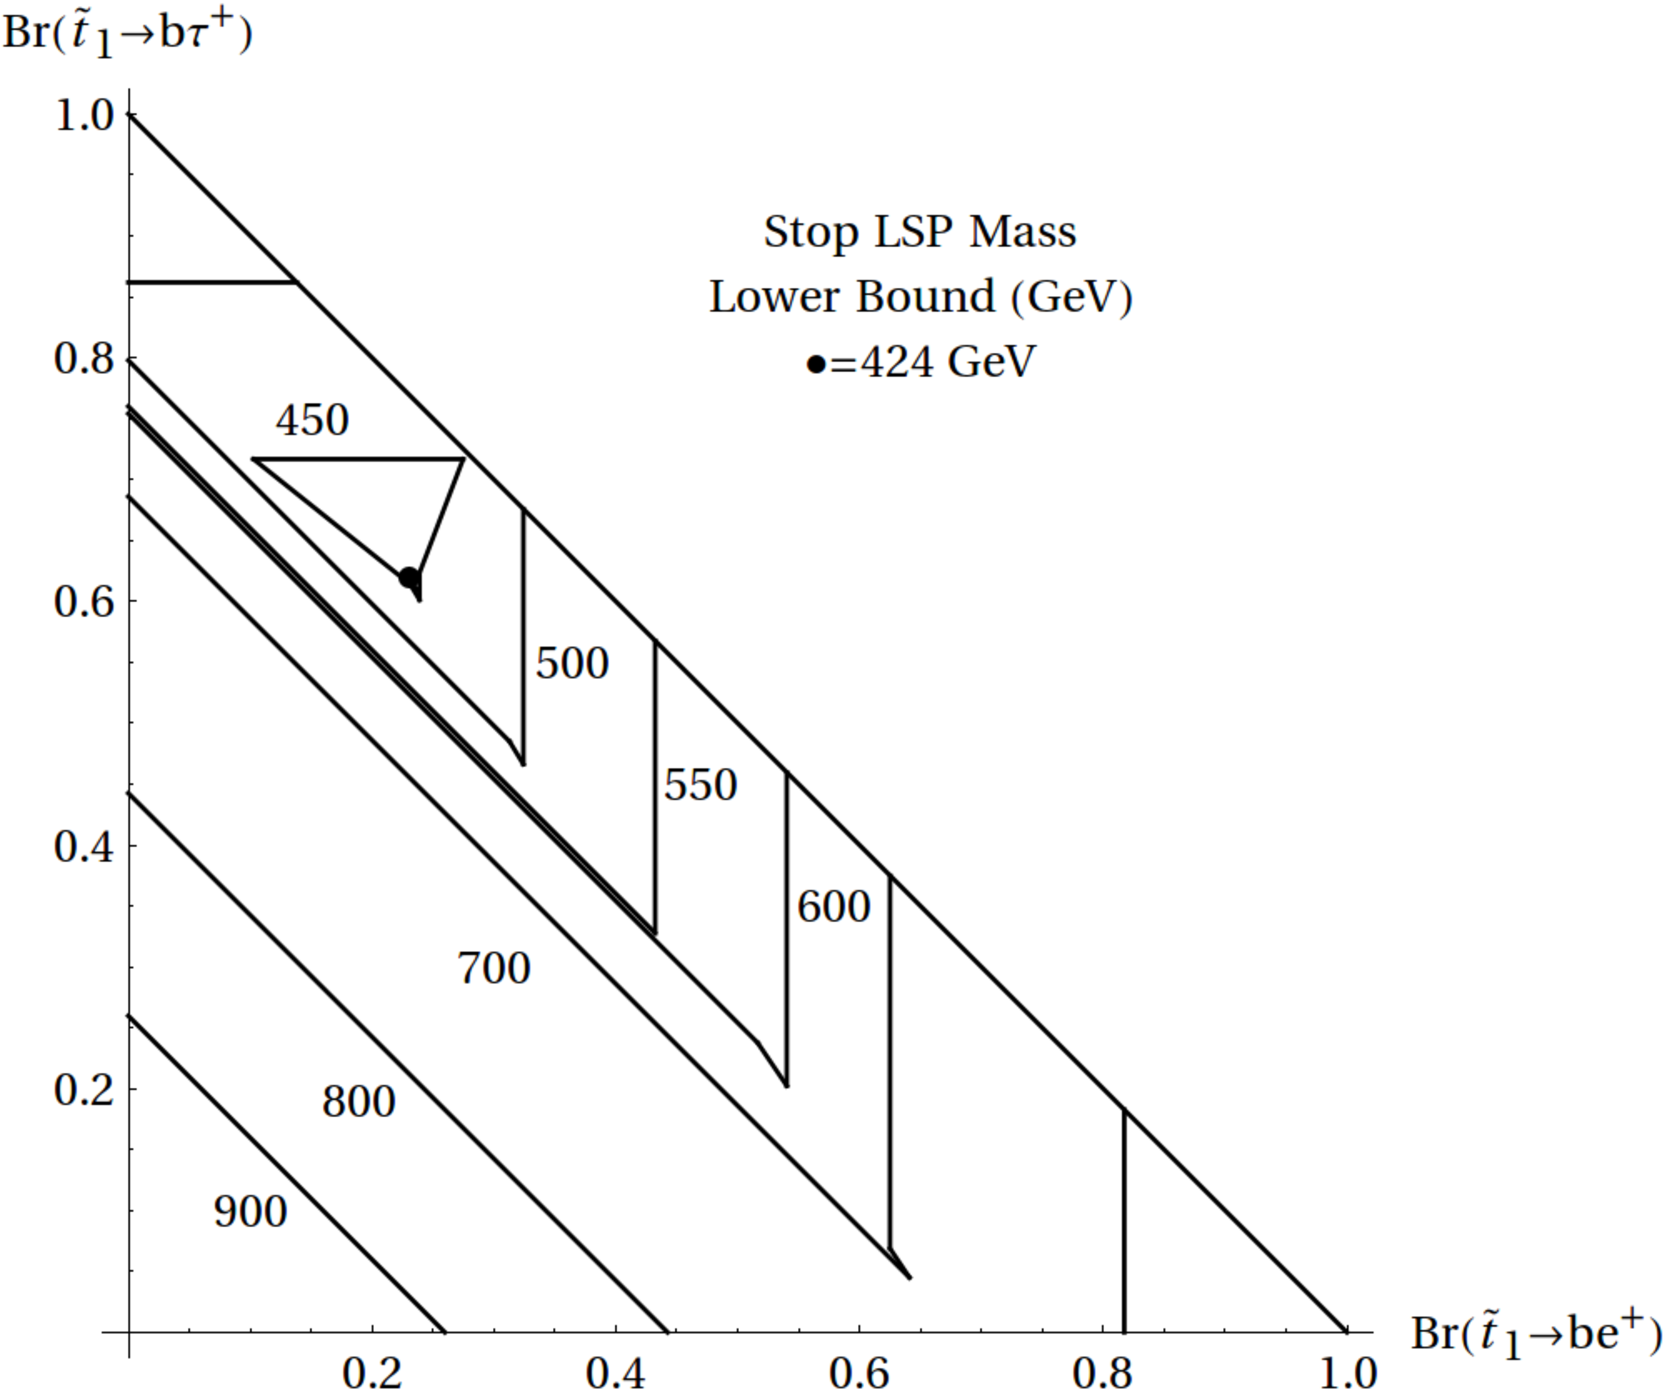
\includegraphics[width=\textwidth]
    {figs/theory/BoundContourPlotNoCombination.pdf}
    \caption{Limits on the stop mass obtained by reinterpreting leptoquark
      searches performed at ATLAS.
      The mass limits assume the stop is the LSP, and decays to a $b$-quark
      and a lepton~\cite{Marshall:2014cwa}.
    }
    \label{fig:pheno_limit}
  }
\end{figure}

